\chapter{System Design}

\section{Back-end Systems}
\subsection{Norton}
Vertex relies on a it's API backend(code-named "Norton"). Norton is written in Python using Flask — a very popular web micro framework. Out of the box Flask comes with far fewer bells and whistles than other similar Python frameworks such as Django however it is much more lightweight and has less dependencies. Flask specialises in preforming as a basic web framework that can be further extended as needed using a plethora of community extensions. Vertex uses one such extension called Connexion. Connexion builds upon Flask and automatically handles HTTP requests in accordance with an OpenAPI file. Connexion automatically routes incoming requests by parsing the requested path and invoking the correct Flask view. The OpenAPI spec has a field called `operationId` which is used to determine which view should be called. This OpenAPI-centric development approach removed the need to manually create individual routing for each endpoint in a typical Flask fashion. It also helped make the code-base more maintainable as it uses the OpenAPI file as the canonical source for the API design. Using the OpenAPI file as the absolute source of truth allows operations such as routing to be updated in one place without the need to alter any additional routing files. A basic Flask / Connexion skeleton can automatically be generated from the OpenAPI file. This was done to generate the initial Vertex prototyping phase as it automatically included relevant documentation from OpenAPI file such as endpoint descriptions as well as expected payloads and return types.


\subsection{Norton Schema}
The Norton API is RESTful by design. There are three main resources in the API scheme.
\begin{itemize}
\item Users: Users consist of an `id` and a `name`. The `id` is used to uniquely identify the user and the name is a
  human-readable intended to be read by other users.
\item Channels: Each Channel has an `id` used to uniquely identify it, a `name` which is displayed to the users and a `type`
  of either `VOICE` or `TEXT` to indicate the channel's use.
\item Messages: Each Message has an associated `author` i.e. the `id` of the User than sent the message, a `channel` i.e.
  the `id` of the Channel the message belongs to, `content` the actual content of the message e.g. "Hello World", an
  `id` each message is given a unique identifier, and a `timestamp` i.e. the number of seconds since the Unix epoch.
\end{itemize}

There are 10 paths within the API. Two used for user creation and authentication i.e. `/login`, `/register` and the rest
are used to access the above resources.

\begin{figure}[h!]
    \centering
    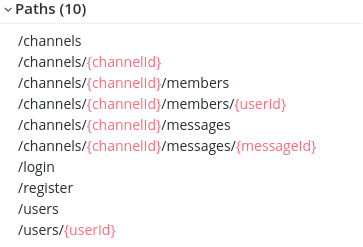
\includegraphics[width=0.7\textwidth]{images/ApiRoutes.png}
    \caption{API Paths}
    \label{image:models}
\end{figure}

New users can be registered by making a HTTP POST request to the `/register` endpoint containing a payload specifying an
unregistered username, and a password. Once registered users can login by posting the same payload to the `/login`
endpoint. When a user is logs in with valid credentials a they are returned a `session\_id` cookie. This cookie is
required to access all non-authentication endpoints and should be presented with all future requests. The same cookie is
used to authenticate with the Notification Messaging System.

The `/channels` and `/users` are very simple endpoints that expose access to the users and channels in the database.
Both endpoints return list of their associated types and can return a single entity if an `id` is specified in the form
`/endpoint/id`.

The users are members of certain channel can be found as a sub-collection of the channel endpoint i.e.
`/channels/id/members` will act similarly to `/users` but will only return users who are members of the specified
channel. The messages in a channel are also a sub-collection of the channel endpoint and can be accessed in a similar
fashion at `/channel/id/messages`

\subsection{Notification Messaging System}
The Notification Messaging System(NMS) is a sub-component of Norton. It runs as it's own process an keeps the server and
clients states in check. When the client first connects to the Norton it fetches the required resources e.g. the
channels available on the server, the messages in a chat, etc. However the client has no way of knowing if the state is
ever updated; NMS solves this. The NMS has a Secure Websocket that client's can listen on for changes in state. If a
change occurs server-side that a client needs to be made aware of it can dispatch a notification to the specific client
to update the state it is missing. For instance if a user joins a channel a notification is dispatched to all other
users of the channel that they need to update their members list for that channel. This system allows for clients to be
inform of state change without needing to consistently poll the database. Messages are dispatched based on the users'
ids. The client authenticates with the Websocket by providing its `session\_id` cookie and is returned a list of
notifications.

\subsection{Notification Structure}
Each notification will be sent as JSON and consist of three key/value pairs:
\begin{enumerate}
\item Target: The target is the User's id that the message is intended for. This is used primarily to route messages to each user. For all intents and purposes the target is mostly irrelevant from the clients perspective.
\item Type: The message type is used to identify the appropriate update method e.g. `get\_channels` would indicate that clients channels need updating and the payload would indicate which channels need refreshing.
\item Payload: The payload is the data needed to complete the update functionality. e.g. a payload of `{"user": 100, "channel": 201}` with a type of `add\_user\_to\_channel` would indicate that user `100` has been added to channel `201`
\end{enumerate}

\begin{tabular}{|l|l|l|l|}
\hline
\thead{Target} & \thead{Type} & \thead{Payload} \\ 
                \hline
101    & add\_user\_to\_channel  & \{“user”: 100, “channel”: 201\}    \\ \hline
101    & create\_channel         & \{“channel”: 1011\}                \\ \hline
106    & delete\_channel         & \{“channel”: 1015\}                \\ \hline
101    & delete\_message         & \{“channel”: 201, “message”: 320\} \\ \hline
101    & remove\_channel\_member & \{“channel”: 999, “message”: 100\} \\ \hline
101    & update\_channel         & \{“channel”: 999\}                 \\ \hline
101    & update\_message         & \{“channel”: 999, “message”: 321\} \\ \hline
\end{tabular}

\begin{figure}[h!]
    \centering
    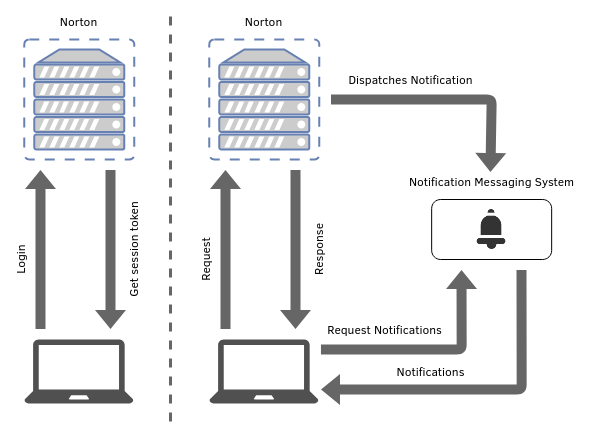
\includegraphics[width=0.7\textwidth]{images/Norton.png}
    \caption{Notification Messaging System}
    \label{image:models}
\end{figure}

\section{Creating Main Business Logic for Vertex}
\subsection{Models}
Vertex uses five models which are implemented from the Norton-API client-stubs. These stubs were generated from OpenAPI specification for the back-end python server, which has been aliased as Norton.
\\ The API stubs live in their own repository outside of the application. To use it in Flutter they are listed as a dependency in the projects 'pubspec.yaml' file.
\\ The business logic makes use of the models to pass data from the view-models to services.
See Figure~\ref{image:models}.

\begin{figure}[h!]
    \caption{Example of Models}
    \label{image:models}
    \centering
    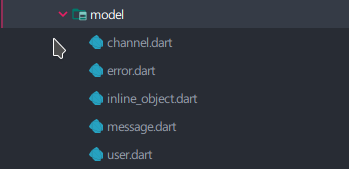
\includegraphics[width=0.7\textwidth]{images/models.png}
\end{figure}

\subsection{View Models}
A view model's purpose is to take data from a source and put it into a presentable form that the UI can interpret.
\\ Vertex uses four view-models to handle CRUD (Create, Read, Update, Delete) operations and update state figure~\ref{image:vertexArch}. To understand how one works see figure~\ref{image:channelViewModel} for a breakdown of the class.

\begin{figure}[h!]
    \caption{Vertex Architecture}
    \label{image:vertexArch}
    \centering
    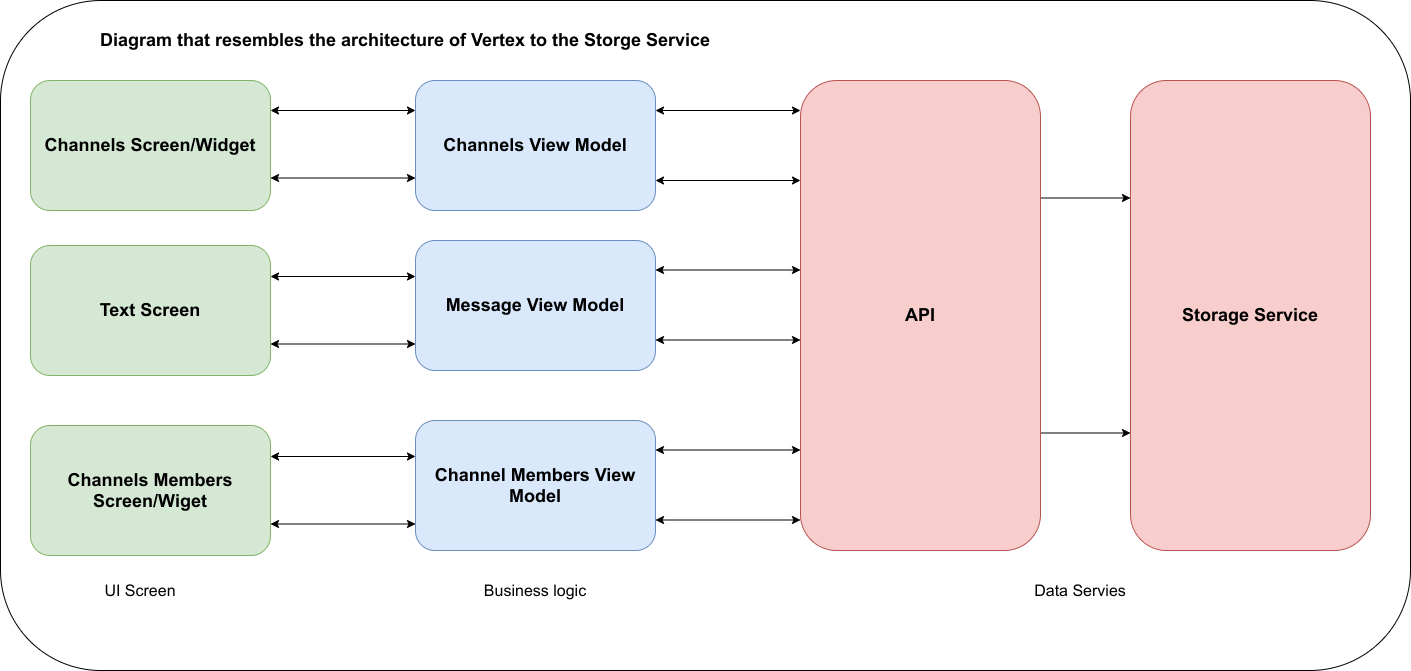
\includegraphics[width=1.0\textwidth]{images/vertex_arch.png}
\end{figure}

\begin{figure}[h!]
    \caption{Channel View Model Code Example}
    \label{image:channelViewModel}
    \centering
    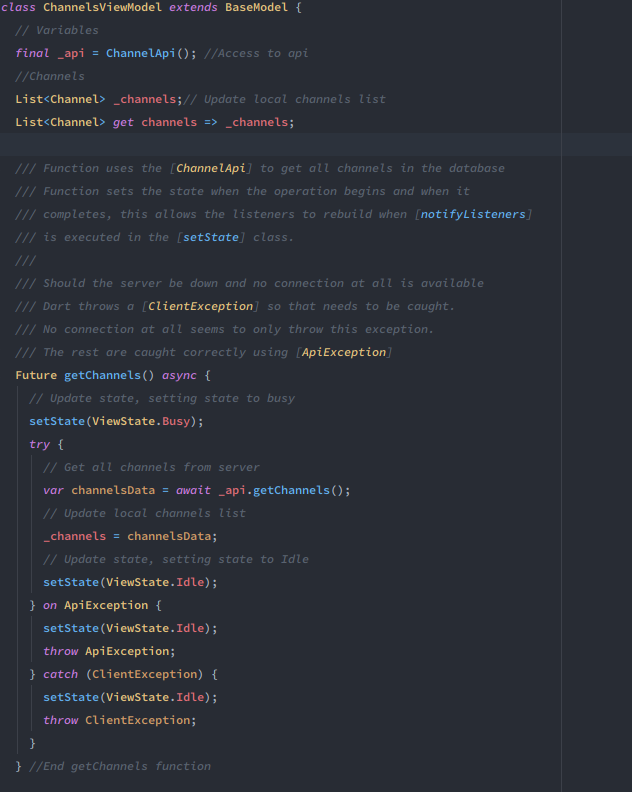
\includegraphics[width=1.0\textwidth]{images/channel_view_model_code.png}
\end{figure}

Figure~\ref{image:channelViewModel} is the ChannelViewModel class. As described in the comments it is the function that gets all the channel data from the server and updates the applications state.
\\\\ Note the following in figure~\ref{image:channelViewModel}: 
\begin{enumerate}
    \item The class is extending a class called BaseModel which is in charge using Change Notifier which provides ‘notifyListeners()’. This allows for widget rebuild.
    \item The API service is declared as \_api, this allows access to the Norton-API-client stubs CRUD functions for Channels.
    \item The Lists store a list of Channels using the Channels model locally so widgets can access its data.
    \item Inside the getChannels() setState() is classed passing ‘ViewState.Busy’, this notifies the listening widgets that an operation is taking place so the widget is able to display a progress indicator. 
    \begin{enumerate}
        \item The channel data is fetched from the server using the API-client stubs.
        \item The local List is updated with the channel data.
        \item setState() is called again setting its state to ‘ViewState.Idle’. This then notifies the listening widget to build with the new data received from the server.
    \end{enumerate}
    \item The final part looks after expectations thrown from the API-client stubs or Dart client exceptions. Should an exception be thrown the UI is updated to reflect the exception in an alert Dialog. 
\end{enumerate}
All other view models are built the same but just in charge or different data or views. In summary, the view models call setState() to update the UI with the new state. This pattern can be used with Streams in Flutter as well but for this application Future functions were used as they are asynchronous.

\subsection{Adding a Services Locator and Injecting Services}
The view-models are injected as a service into the application at run time with the help of a package called ‘get\_it’. \textit{“This is a simple Service Locator for Dart and Flutter projects with some additional goodies highly inspired by Splat. It can be used instead of InheritedWidget or Provider to access objects e.g. from your UI.”} [ADD ME: 1]. This allows for access to the view-models anywhere in the application by calling the locatorGlobal and the name of the service you wish to access. ‘get\_it’ is another dependency which is set in the applications pubspec file. 
\\ All services are registered as a Lazy Singleton, meaning it is created when it first gets invoked and it will always receive the same instance back. This is important as the view-models store data locally in Lists.
\begin{figure}[h!]
    \caption{Example of GetIt Class}
    \label{image:getItClass}
    \centering
    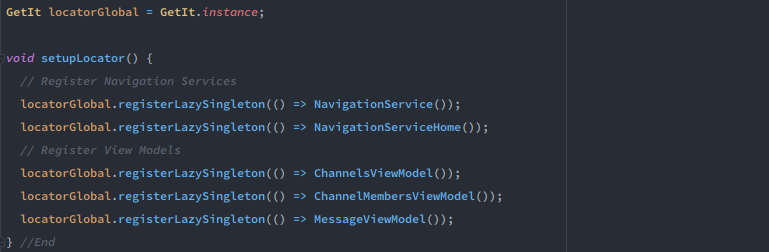
\includegraphics[width=1.0\textwidth]{images/get_it_class.png}
\end{figure}
\\\\Note the following in figure~\ref{image:getItClass}:
\begin{enumerate}
	\item Instance of ‘GetIt’ is created
	\item Navigation service View-models are registered
	\item In main.dart the main() function will call setupLocator() before calling runApp()
\end{enumerate}

\subsection{Implementing Provider}
Implementing Provider into the application is only a small part of the overall state management architecture implementation. Provider is another dependency that is listed in the applications pubspec.
\\ Provider has a widget called ChangeNotifierProvider. It is the widget that listens for changes in the view-model classes that extend ChangeNotify. With the use of ChangeNotify Provider and ChnageNotify in the application a widget/class called BaseView was created to aid in the process of fetching data and updating state. This class was adapted from a Flutter developers implementation of Provider and state management[ADD ME: 2]. Figure~\ref{image:baseViewClass} is a breakdown of the class.
\begin{figure}[h!]
    \caption{Example of BaseView Class}
    \label{image:baseViewClass}
    \centering
    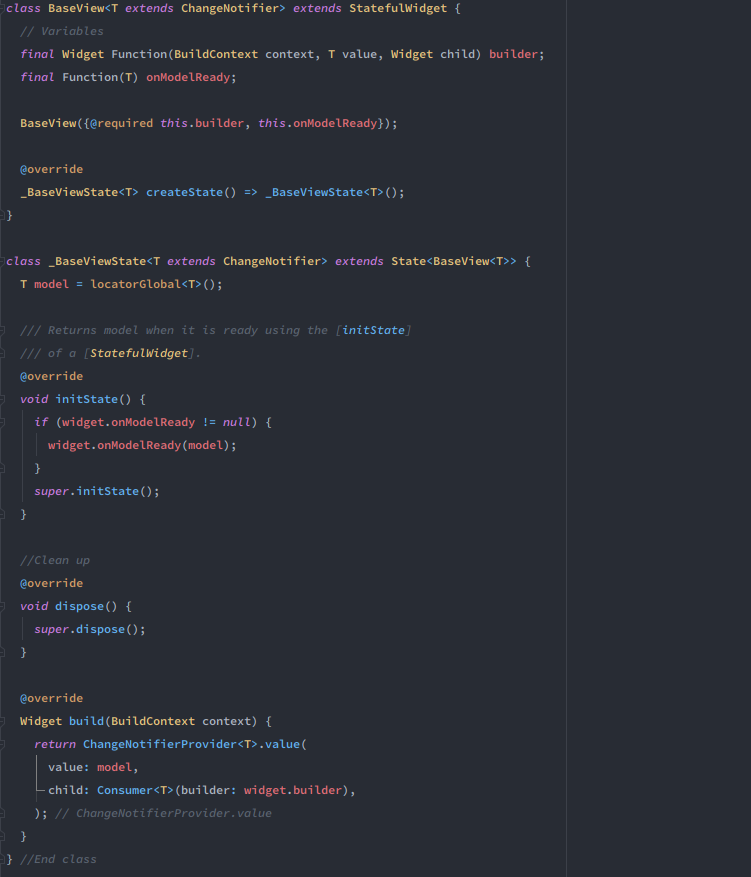
\includegraphics[width=1.0\textwidth]{images/base_view_class_code.png}
\end{figure}
\\\\Note the following in figure~\ref{image:baseViewClass}:
\begin{enumerate}
	\item The class converts a widget into a Stateful widget so the onInit function can be used to pass the model back to use in a callback function.
	\item Function(T) returns the model, this now gives access to the function inside that model class.
	\item The \textit{onModelReady} can now be used to notify the UI element that can display the data or display a progress bar depending on the BaseModel.state, the class that notifyListeners.
	\item The Widget Build function returns Providers ChangeNotifierProvider function with a value, the value being the view model and the child being the Consumer which has a build function. 
\end{enumerate}

\section{Integration With UI}
So with Provider and now the BaseView Widget it can all be put together in one of the view classes to retrieve data. Figure~\ref{image:messageViewBuilder} is a breakdown of how it works in the text chat view with message data:

\begin{figure}[h!]
    \caption{Example of MessageView Builder}
    \label{image:messageViewBuilder}
    \centering
    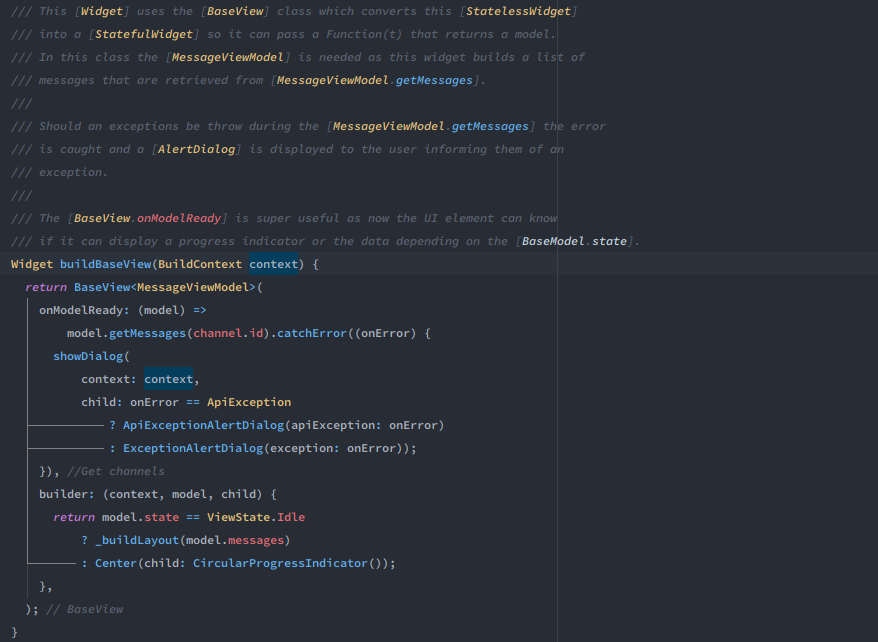
\includegraphics[width=1.0\textwidth]{images/messge_view_builder_with_model.png}
\end{figure}

Note the following in figure~\ref{image:messageViewBuilder}:
\begin{enumerate}
	\item Firstly the BaseView Widget is called passing it the view model that is needed, in this case, MessageViewModel.
	\item model.getMessages(channel.id) in the onModelReady calls the getMessages function from the view-model MessageViewModel. Should an error occur an exception dialog will be displayed to the user.
	\item The builder will return the \_buildLayout() Widget if the model.state is Idle else if will display a progress indicator until the model is ready.
	\item The \_buildLayout() now has the data needed to build its UI.
\end{enumerate}

\subsection{Handling State For WebRTC}
\label{handleStateWebRTC}
The state management is handled a little differently for WebRTC class due to a WebSocket being used to send and receive messages between the WebRTC signalling server. Voice and Video class handle state the same way just in different classes.
\\ When a user wishes to start a video call, the UI class creates an instance of the Signaling class, this class is in charge of connecting to the signalling server, gathering peer data, processing message events and setting up calls with peers when a peer is invited. See Figure~\ref{image:videoSignallingConnectFunc}.
\begin{figure}[h!]
    \caption{Example of Video and Signalling Connection Function}
    \label{image:videoSignallingConnectFunc}
    \centering
    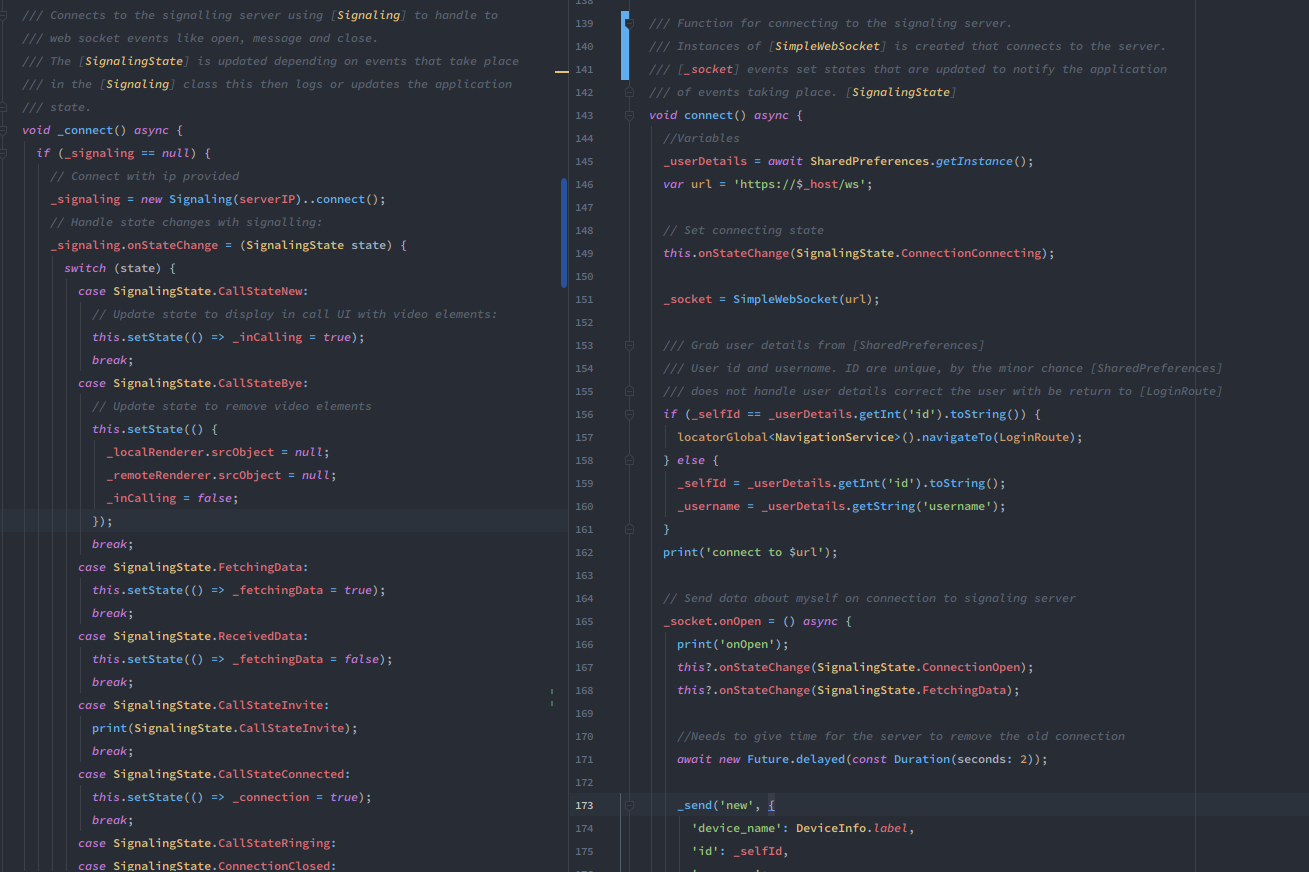
\includegraphics[width=1.0\textwidth]{images/video_and_signalling_connect_fcuntions.png}
\end{figure}

Note the following in figure~\ref{image:videoSignallingConnectFunc} on the left side:
\begin{enumerate}
	\item The Video UI class creates a new instance of the Signalling class passing it the server IP address.
	\item The Video UI class uses the callback function onStateChange declared in the Signalling class to listen for SignallingState changes. When an event is triggered in the Signalling class the Video UI state is updated depending on the SignallingState passed back in the callback function.
\end{enumerate}

Note the following in figure~\ref{image:videoSignallingConnectFunc} on the right side:
\begin{enumerate}
	\item The initial state is set to SignalingState.ConnectionConnecting, this Notifies the UI that the Signalling class is connecting to the WebRTC signalling server.
	\item An instance of SimpleWebSocket created passing it the URL to connect to the WebRTC signalling server.
    \item When the socket opens the connections to the server two new SignallingStates are set, \textit{SignalingState.ConnectionOpen} to notify of the connection successfully opened and \textit{SignallingState.FetchingData} to notify the UI its gathering data from the server, this allows the Video UI class to display a progress bar until the data is received back and the SignallingState is set to \textit{SignallingState.ReceivedData}. All messages that are received are processed accordingly and the appropriate state is set.
\end{enumerate}

\subsection{Implementing Bloc Pattern with Authentication Service for Login \& Register}
The Login and Register components of the application were developed using the Bloc pattern, which worked well with the view and the business logic, as it stream-lines events like navigation and form validation, which is the main purpose of the login and register views. The stream events made it easy to implement an Authentication State listen which would manage logged in access to the application depending on the login request result.
\\ Figure~\ref{image:authServiceClass} defines a Broadcaster/Observable object that can notify its Subscribers of any changes of its authentication state, whether logged in or not. Normally get\_it would be used to inject the service into the application, or the Redux package, but for the applications needs manually implementing it fit the design better.

\begin{figure}[h!]
    \caption{Authentication Service Class Example}
    \label{image:authServiceClass}
    \centering
    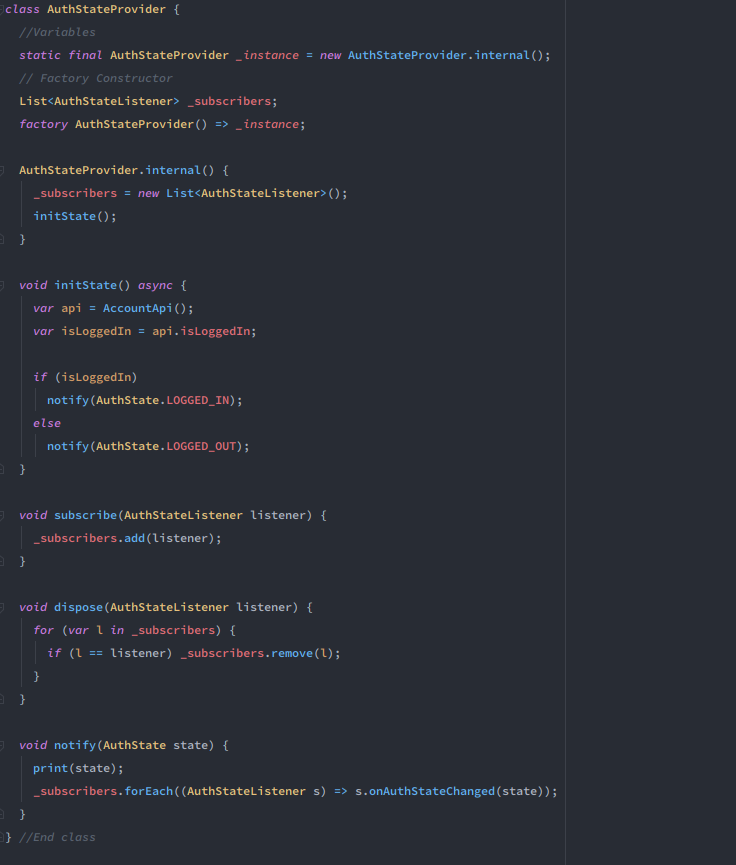
\includegraphics[width=1.0\textwidth]{images/authentication_service_class.png}
\end{figure}

Note the following in figure~\ref{image:authServiceClass}
\begin{enumerate}
    \item A factory constructor is declared at the top of the class using Dart's built factory constructor. This allows other classes to retrieve an instance of the class.
    \item initState() declares an instance of the AccountApi(), which are the client-stubs for the server that allow access to the isLoggedIn variable in the AccountApi() class. This variable is set depending on the result of a login being successful or not. The notify function is called where it will update each subscriber if the user is logged in or not.
    \item The subscribe() adds a new listener to the list so they can be notified of changes in login.
    \item The dispose() will remove a listener from the list.
\end{enumerate}
Referring back to the Bloc pattern, figure~\ref{image:loginViewPresenter} represents the same set up for both the Login and Register components. For the purpose of demonstration only one is displayed. Figure~\ref{image:loginViewPresenter} shows the login view presenter.

\begin{figure}[h!]
    \caption{Login View Presenter}
    \label{image:loginViewPresenter}
    \centering
    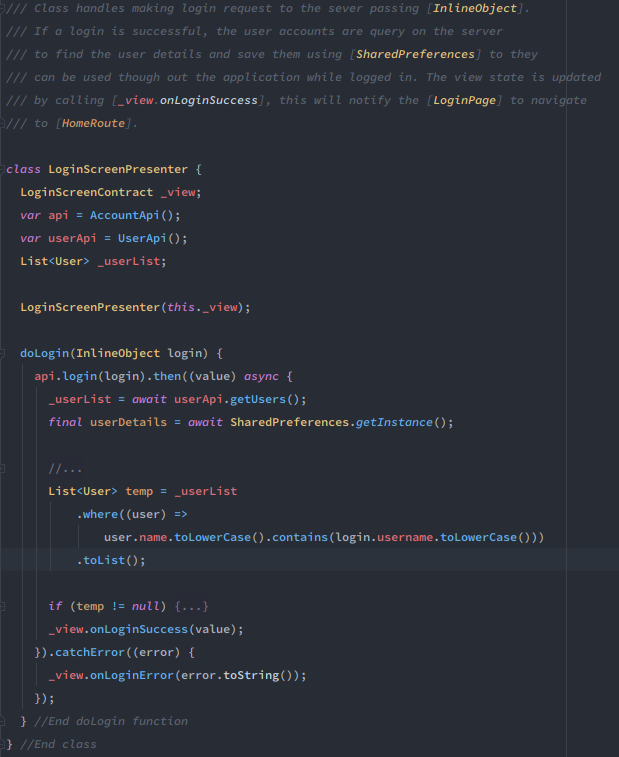
\includegraphics[width=1.0\textwidth]{images/login_presenter_class.png}
\end{figure}

Note the following in figure~\ref{image:loginViewPresenter}:
\begin{enumerate}
    \item The class defines an interface for the LoginView and a presenter that will handle all the business logic specified to LoginView.
    \item An instance of the AccountApi() is declared as a login request will need to be made to authenticate an account with the server.
    \item User account is fetched after a login is successful and details are stored.
\end{enumerate}

Figure~\ref{image:loginViewClass} and figure~\ref{image:loginBloc} breakdown the login view class with the implementation of authentication service and Bloc pattern. 

\begin{figure}[h!]
    \caption{Login View Class}
    \label{image:loginViewClass}
    \centering
    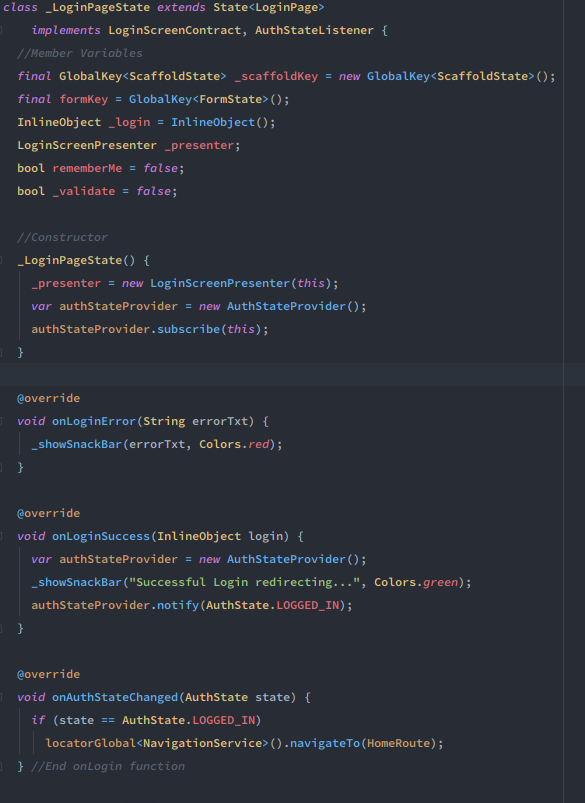
\includegraphics[width=1.0\textwidth]{images/login_view_class_1.png}
\end{figure}

\begin{figure}[h!]
    \caption{Login Bloc}
    \label{image:loginBloc}
    \centering
    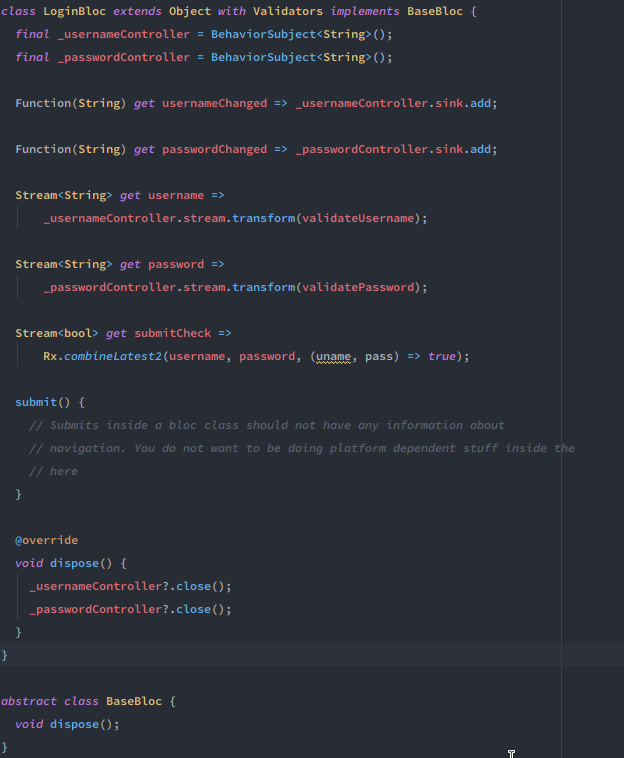
\includegraphics[width=1.0\textwidth]{images/login_bloc.png}
\end{figure}

Note the following in figure~\ref{image:loginViewClass}:
\begin{enumerate}
    \item The LoginScreenContract abstract class is implemented which imports its function onLoginSuccess() and onLoginError() these function will now be able to update the views state depending on the business logic in the LoginScreenPresenter class.
    \item AuthStateListener is also implemented which imports onAuthStateChanged, this now allows the login state to be updated if a login is successful in the onLoginSuccess(). The user is then navigated to the HomeRoute using the navigation service.
    \item The rest of the class builds the form UI for users to login with their details.
\end{enumerate}

Note the following in figure~\ref{image:loginBloc}:
\begin{enumerate}
    \item The LoginBloc class is used to read in the stream on data from the form text controller, validate it using the validators and return true to the StreamBuilder in the LoginView class where its state will update.
\end{enumerate}
The Bloc pattern worked very well when implemented for the login and registration but its overall design compared to the Provider architecture required more code for the same outcome so ultimately Provider fit the applications needs better for state management.

\subsection{Navigation Implementation}
\label{NavSection}
Vertex started out as an application that was going to be on iOS, Android and Web, so with that navigation took some planning and consideration as it would need to be a mix of pop on and off the stack using widgets as well as routing.
\\ Initially the app started out with the pop on pop off theme while developing the login, register and main home page. While this worked, as more views were implemented, and data needed to be passed around the app, it needed to be revisited. It quickly became apparent that that navigation was needed where the BuildContext was not always available.
\\ To overcome this issue a navigation service was created which would use a GlobalKey that is unique across the app. A GlobalKey provides access to other objects that are associated with those elements, such as the BuildContext. For Stateful Widgets, global keys also provide access to its State. This method of navigation was much more useful so it became incorporated across the application. 
\\ Two Navigation services were created:
\begin{enumerate}
    \item NavigationService which handles global routes by their route name.
    \item NavgationServerHome which handles internal routes that only buttons interaction can be used to navigate to its routes. These routes require data models to be passed with them.
\end{enumerate}

\begin{figure}[h!]
    \caption{Navigation Service}
    \label{image:navService}
    \centering
    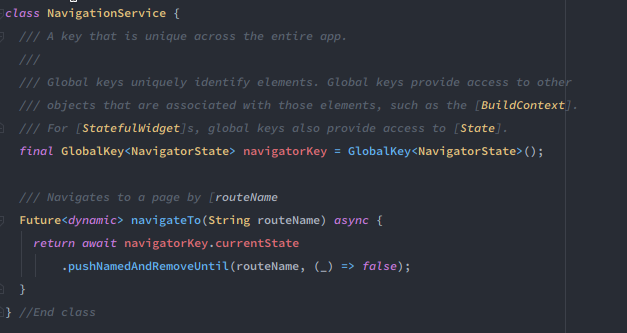
\includegraphics[width=1.0\textwidth]{images/navigation_service_class.png}
\end{figure}

Note the following in figure~\ref{image:navService}:
\begin{enumerate}
    \item GlobalKey for NavigatorState is create.
    \item Future function navigateTo requires an arguments routeName which is the route name that is going to be navigated too.
\end{enumerate}

NavigationServiceHome is the same, only it always can accept a dynamic argument as well. This dynamic argument is mostly a channel data model. The two services are registered in locator.dart file using 'get\_it' where they are accessible anywhere throughout the application using locatorGlobal<NavigationService>().navigateTo(routeName).
\\ A class called router.dart has two functions declared inside it which are switch statements:
\begin{enumerate}
    \item generateRoutes, which allows access to the HomeRoute, SettingsRoute, LoginRoute and RegisterRoute through the UI Widgets onGenerateRoute declared in the Widget.
    \item internalRoutes which allow access to the MessageRoute, VoiceChannelRoute, LandingPageRoute, and EditChannelRoute through the HomeLayoutTemplate Widgets onGenerateRoute.
\end{enumerate}
The internal routes lead into section~\ref{UI} and why it was needed.

\subsection{User Interface}
\label{UI}
The user interface started out with some basic views that would change when you navigate to another page that's fine it works but it didn't fit the need of the application. With the app being a communication application with different channels it became apparent that a UI would need to be designed where one section of the view could stay the same for the most part while other parts were capable of being updated with a different view on user interaction. See figure~\ref{image:vertexHomePage} 
\begin{figure}[h!]
    \caption{Vertex Home Page}
    \label{image:vertexHomePage}
    \centering
    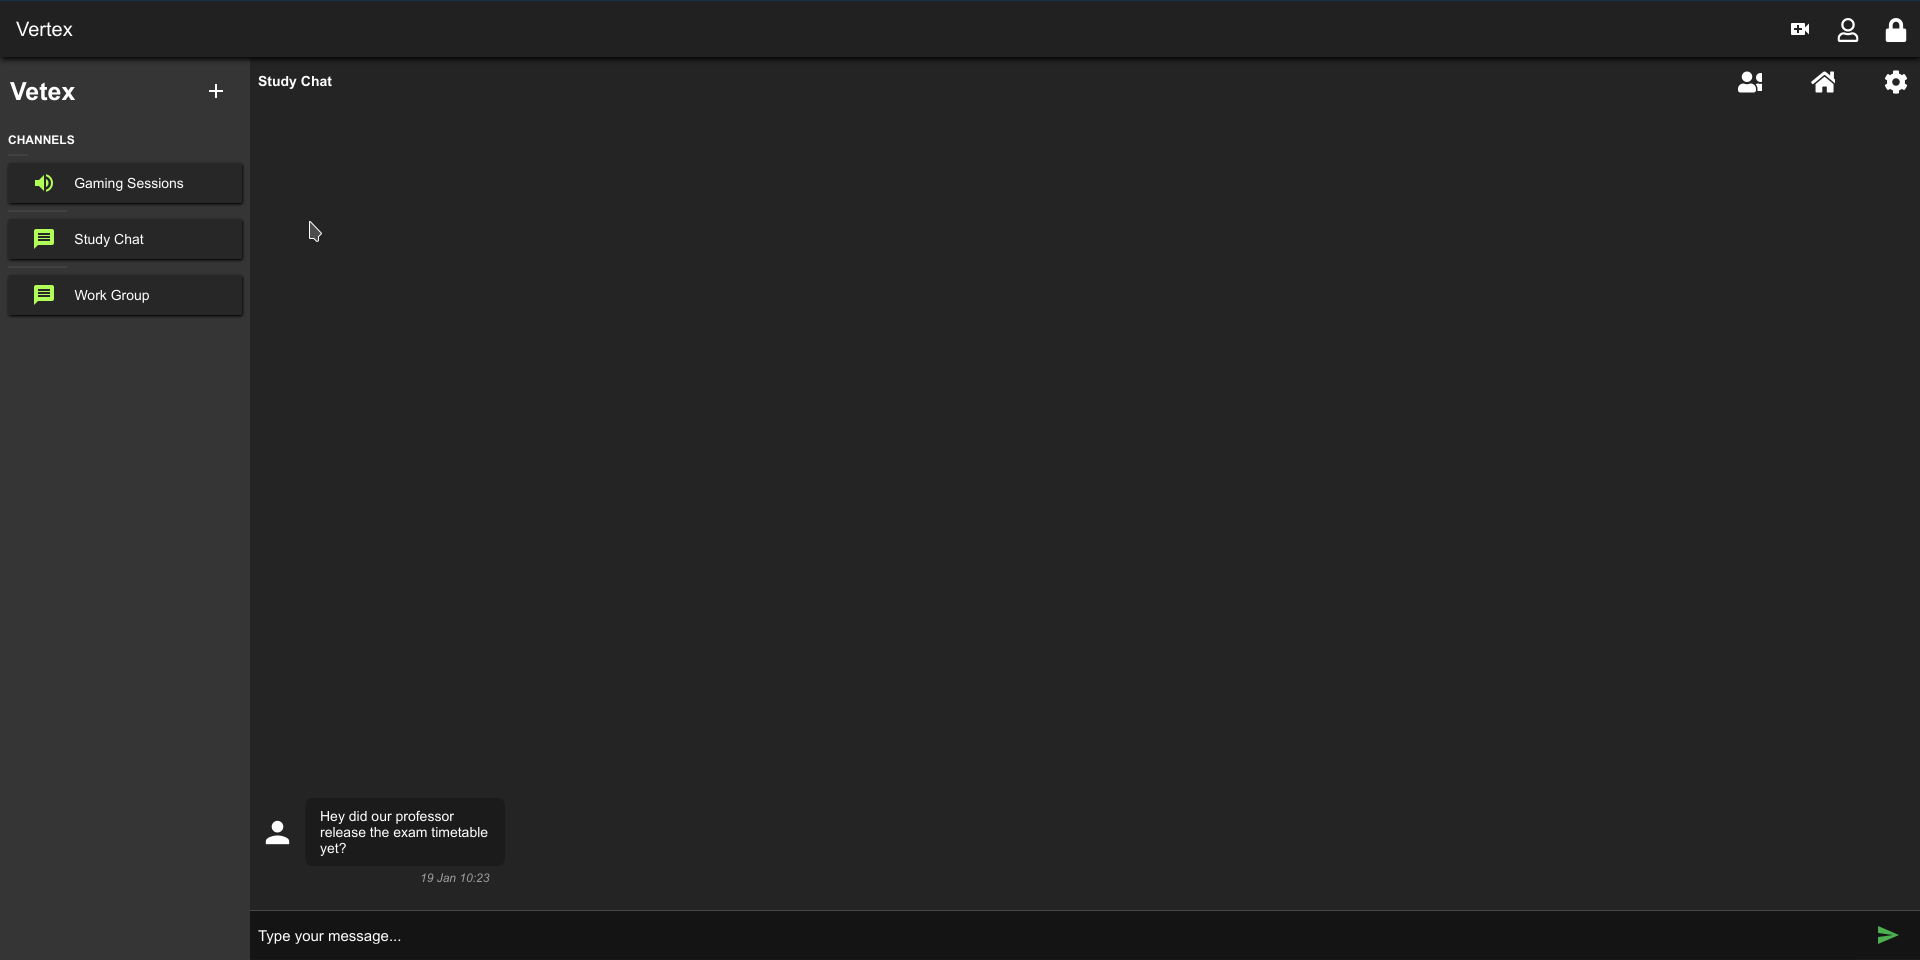
\includegraphics[width=1.0\textwidth]{images/vertex_homehome_view.png}
\end{figure}

Note the following in figure~\ref{image:vertexHomePage}:
\begin{enumerate}
    \item While the user is on the home page they can navigate between channels they select on the right and the left side rectangle will update its view to reflect the channel the user has selected.
    \item The List of channels will stay displayed on the right unless the user navigates to setting, video call or logout which are the three button icons on the very top right of the figure. The icon buttons below that allow the user view a list of members in the channel they are currently in, navigate to home which is a home view inside the rectangle on the right or display settings for that channel whereby a user can update the channel name or delete the channel. 
\end{enumerate}

To achieve this user interface design, a layout template was designed that would handle its own navigation routes, that is where the internalRoutes function talked about in the section~\ref{NavSection} comes into play. The layout allows the Landing view, message view and voice call view to be rendered inside that template while keeping the external view the same.
\\ With the application being developed for both mobile platforms and web a responsive design needed to also be implemented into the application so that the above views would render correctly on all platforms. A package called responsive\_builder developed by the Flutter community was used to achieve the layout across multiple platforms and screen sizes.

\begin{figure}[h!]
    \caption{Settings Folder Tree}
    \label{image:settingsFolderTree}
    \centering
    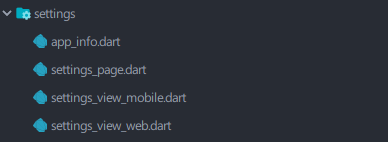
\includegraphics[width=0.7\textwidth]{images/settings_folder_tree.png}
\end{figure}

\begin{figure}[h!]
    \caption{Settings UI Widget}
    \label{image:settingsUIWidget}
    \centering
    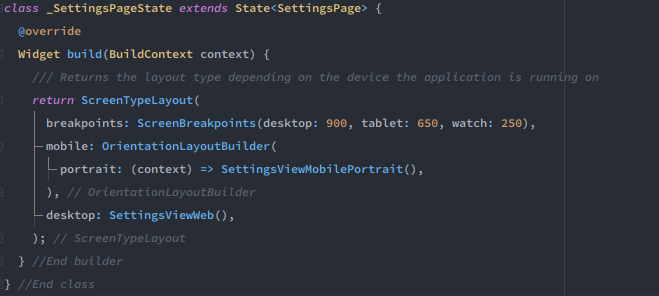
\includegraphics[width=1.0\textwidth]{images/settings_ui_widget.png}
\end{figure}

Note the following in figure~\ref{image:settingsFolderTree} and figure~\ref{image:settingsUIWidget}:
\begin{enumerate}
    \item The settings folder holds settings\_page which is displayed in figure~\ref{image:settingsUIWidget}, that returns either settings\_view\_mobile or settings\_view\_web.dart depending on the screen layout and size.
\end{enumerate}

The main home widgets handle building the UI the same way. With the responsive build now implemented, when a browser window is resized the application will respond to that change and rebuild the UI. See figure~\ref{image:mainWindow} and figure~\ref{image:mainWindowOpenDrawer}. It may not seem like much but a lot of planning around how to implement this was very much needed as the application was going to be running on a browser as well as mobile devices which all can vary in screen size.

\begin{figure}[h!]
    \caption{Home Page}
    \label{image:mainWindow}
    \centering
    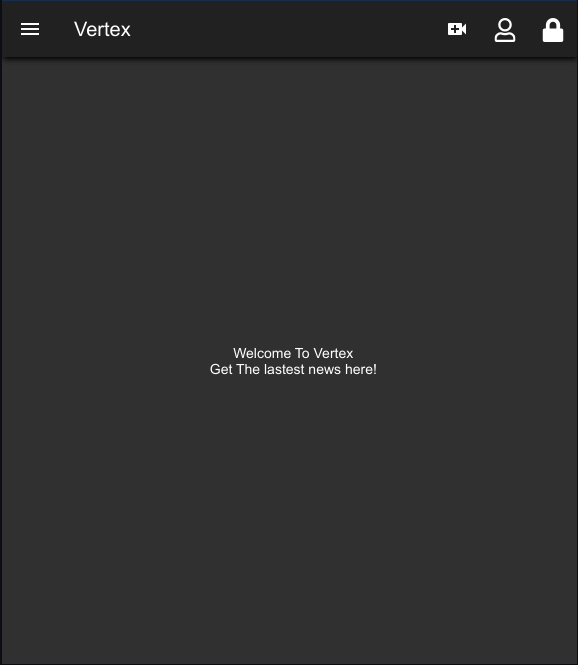
\includegraphics[width=1.0\textwidth]{images/resized_window_main.png}
\end{figure}

\begin{figure}[h!]
    \caption{Home Page with Open Navigation Drawer}
    \label{image:mainWindowOpenDrawer}
    \centering
    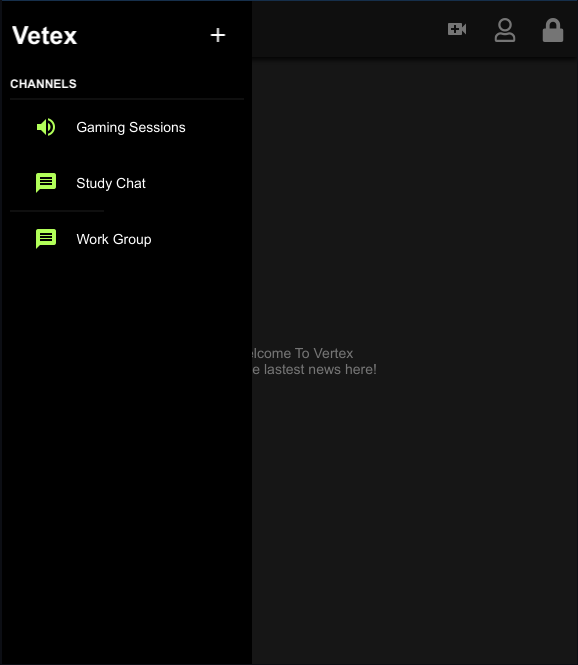
\includegraphics[width=1.0\textwidth]{images/resized_window_drawer_open.png}
\end{figure}

\subsection{WebRTC Signalling Server}
As previously discussed in section~\ref{webRTCTR},  establishing a WebRTC connection between two devices requires a signalling server to resolve how peers can connect over the internet. A signaling servers job is to act as a link in the middle of two peers that wish to connect to each other. WebRTC doesn't specify a transport mechanism for signaling information so a WebSocket is used to send and receive messages from client to server.
\\ The signalling server does not need to understand or interpret the signalling data. SDP data is sent to enable WebRTC class but the socket doesn't need to worry about understanding it. What is important when the ICE instructs the websocket to send signaling data to another peer. When the other peer receives information  it knows how to receive the information and deliver it to its own ICE subsystem. All the signalling server has to do is channel the information back and forth, the context doesn't matter at all to the signalling server.
\\ The WebSocket sends information between client and server using a JSON string. The server processes several event types that are in the JSON message such  as “new” which will add a new peer(connection) to the websockets array list and return the list to all peers connected, candidate which is a peer that wishes to communicate with another and bye which will end a call between two peers.

\subsubsection{Signalling Protocol Design}
Now that the websocket is able to exchange messages a protocol needs to be defined of how the message will look. A stringified JSON object is used to communicate with its clients, this means the websockets message will also be in JSON format with implementation of what type of message it is and any additional data needed.

\subsubsection{Peer Connection Exchange}
Vertex displays a list of peers connected to the websocket as they are peers that wish to commute. When a new client connects to the websocket it will send a message to the server with information about itself. The messages have the following fields:
\begin{itemize}
    \item type - The message type: “new”
    \item device\_name - The type of device the peer is on and connected with to the server.
    \item username - The peers username. In a normal design this can be left out. For the sake of Vertex it was easier to distinguish who is trying to connect to who and who's in a call with you.
    \item user\_agent - This has information about the operating system the peer is using.
\end{itemize}
When a message type “new” is received, the connection array is updated with the new connection and the new connection peer information is sent to all currently connected peers.
\\ This allows the client application to update its UI with available peers to connect to. 

\subsubsection{ICE Candidate Exchange}
Peers need to be able to exchange ICE candidates to be able to create a direct connection between them. An 'icecandiate' event is sent to the RTCPeerConnection to complete the process of adding a local description using 'pc.setLocalDescription(offer)'.
\\ Once two peers agree on a mutually-compatible candidate, that candidate SDP is used by each peer to open a connection, by which media is sent between each of them so they can communicate.
\\ Each ICE candidate is sent to the other peer by the following message with these fields: 
\begin{itemize}
    \item type - candidate.
    \item to - id of peer being sent to.
    \item id - id of the peer sending the candidate message.
    \item candidate - SDP candidate string, with information describing a proposed connection method. This message is just passed onto the peer with the id that is equal “to”.
\end{itemize}

Each ICE message suggests a communication protocol (TCP or UDP), IP address, port number and connection type along with other information needed to link two computers together.

\subsubsection {Connection Termination}
This is not an essential part of the protocol, but rather to allow the clients to update the state of their application when a call ends
\begin{itemize}
    \item type - bye
    \item session\_id - This is made when two peers connect to each other. It is both of their ids with a - to delimit them.
    \item from - id of the peer that sent the bye message.
\end{itemize}

The session is split up so two ids are available and a “bye” message is sent to both.
\\ The WebRTC signalling server was developed using Typescript and Node, getting into the code firstly a secure websocket(WSS) needed to be defined as WebRTC requires a secure connection to exchange data between peers that are looking to communicate. 
\\ To create a secure websocket a HTTPS server needs to be created first with SSL
Certificates, this server will just a text message if routed to in a web browser. 

\begin{figure}[h!]
    \caption{WebRTC Signalling Server Code Example}
    \label{image:webRTCSigServCode}
    \centering
    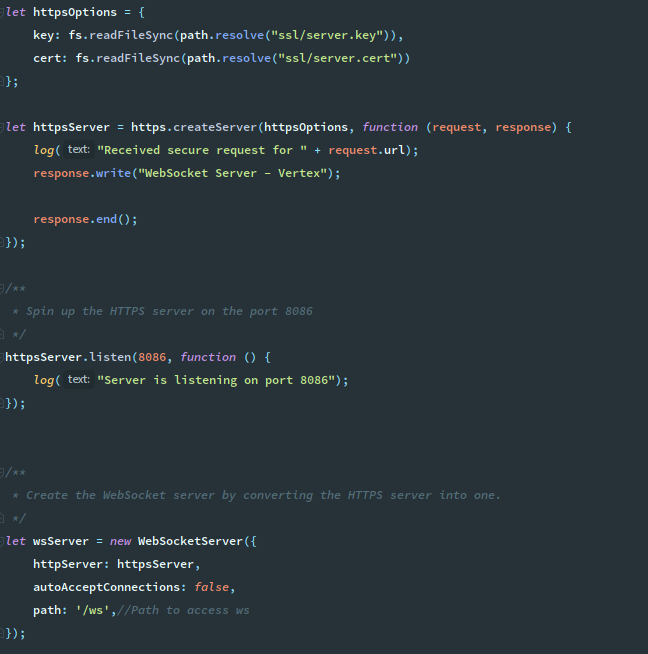
\includegraphics[width=1.0\textwidth]{images/webrtc_signalling_server_code.png}
\end{figure}

Note the following in figure~\ref{image:webRTCSigServCode}:
\begin{enumerate}
    \item The SSL certs are read.
    \item A HTTPS server is created with a response message.
    \item The HTTPS server is started on port 8086
    \item The HTTPS server is passed into a WebSocket to create a secure web socket that is capable of allowing WebRTC clients to connect to it.
\end{enumerate}

\begin{figure}[h!]
    \caption{WebRTC Signalling Server  Switch Code Example}
    \label{image:webRTCSigServSwitchCode}
    \centering
    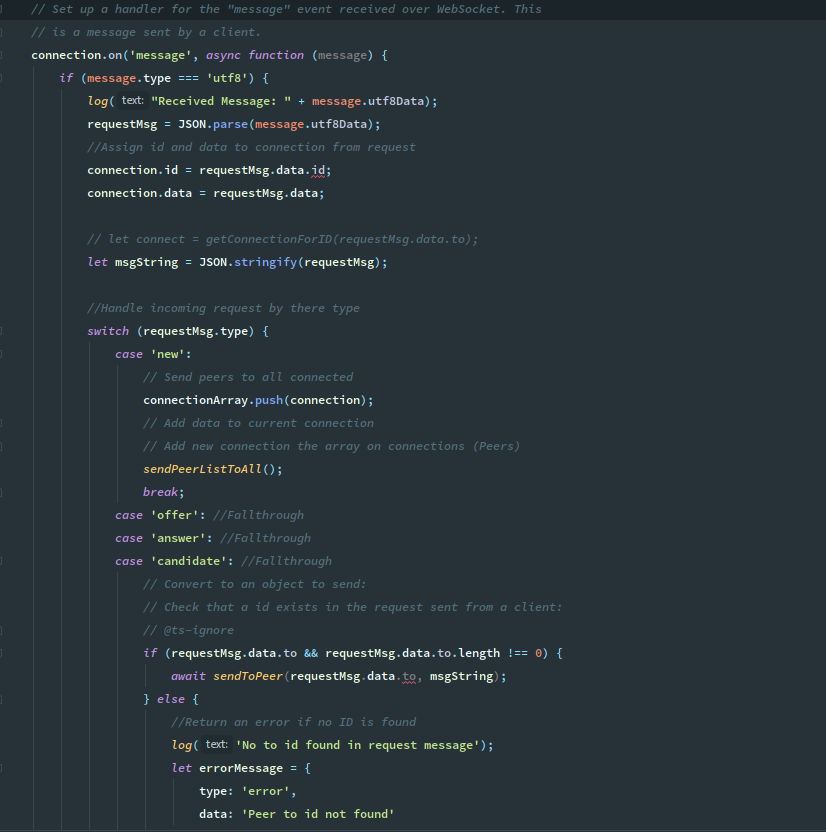
\includegraphics[width=1.0\textwidth]{images/signalling_server_switch_code.png}
\end{figure}

Note the following in figure~\ref{image:webRTCSigServSwitchCode}:
\begin{enumerate}
    \item Connections to the websocket are assigned if that are passed in the message from the client. The data in the message is also assigned to the connection.
    \item The switch statement handles the message type and processes the message accordingly.
    \item In the candidate case, a “to” id is checked for in the request message from a peer, the candidate data is then sent onto that peer by looping through the connections array and finding the connection that equals the “to” id.
\end{enumerate}

\subsection{WebRTC Implementation in Flutter}
Implementing WebRTC was aided with the flutter-webRtc\cite{FlutterWebRTC}, developed by CloudWebRTC\cite{cloudWeb}. The package supports Android, iOS, Web and MacOS and its feature set for all those platforms are:
\begin{enumerate}
    \item Audio/Voice Calls
    \item Data Channel
    \item Screen Capture
\end{enumerate}
The package is imported into the project by listing it as a dependency in the applications pubspec file. CloudWebRTC have a flutter-webrtc-demo available on their git repository\cite{webrtc-demo} which code from there was based on and adapted to use in Vertex.
\\ Vertex allows two peers to communicate via video call or voice call, in order for peers to communicate they must first connect to a signalling server. 
\\ As talked about in section~\ref{handleStateWebRTC}, a websocket is used to connect Vertex to the signalling server to send and receive messages. 
\\ When the client connects to the server it sends information about itself to the server so other peers can see it listed as somebody to connect to. 

\begin{figure}[h!]
    \caption{Connect Message Example}
    \label{image:connectMessageExample}
    \centering
    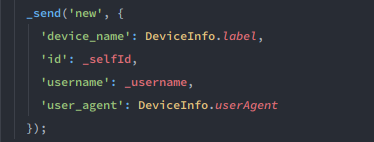
\includegraphics[width=0.7\textwidth]{images/new_connnect_message.png}
\end{figure}

The local peer and a list of connected peers are returned from the server where the data can be used to display the peers available in a list view. This view allows a peer to invite another peer listed in the view as seen in figure~\ref{image:voiceCallLobby}. When a peer is invited a peer connection is set up and a message with candidate information is sent onto the server where that is sent to the peer that was invited to the call.

\begin{figure}[h!]
    \caption{Voice Call Lobby}
    \label{image:voiceCallLobby}
    \centering
    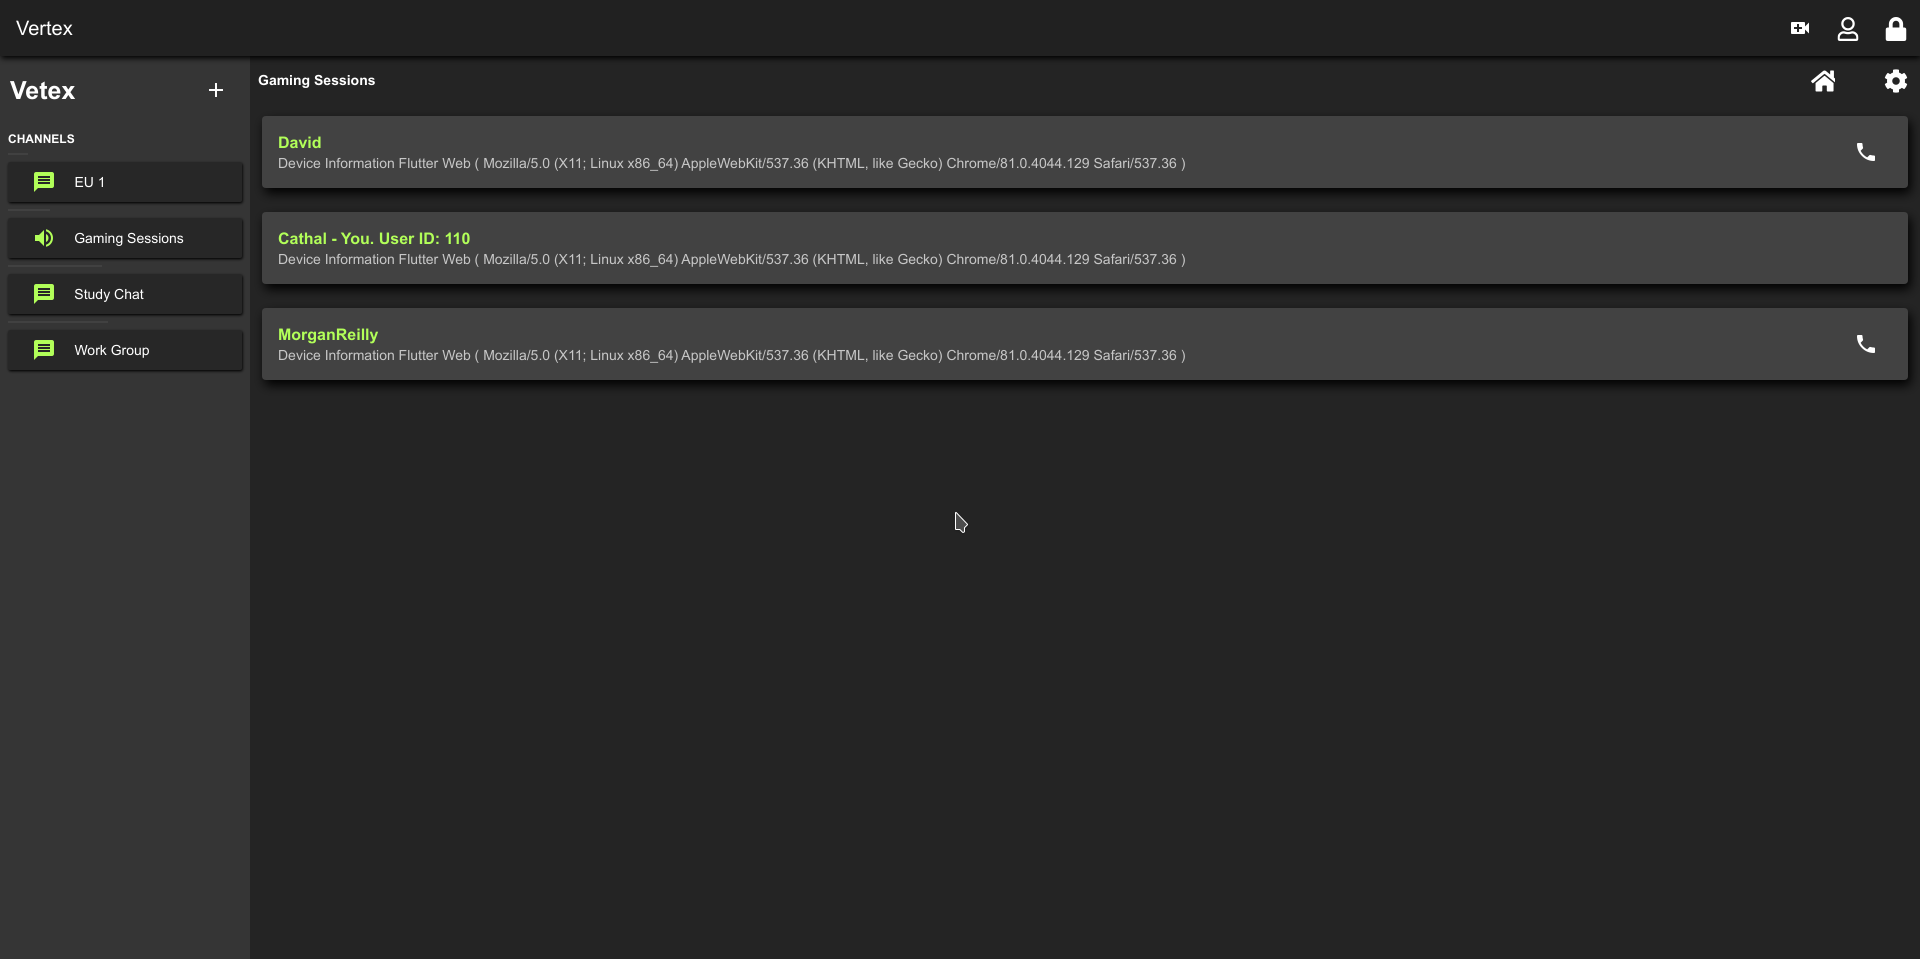
\includegraphics[width=1.0\textwidth]{images/voiceCallLobby.png}
\end{figure}

\begin{figure}[h!]
    \caption{Peer Connect Function}
    \label{image:peerConnectFunction}
    \centering
    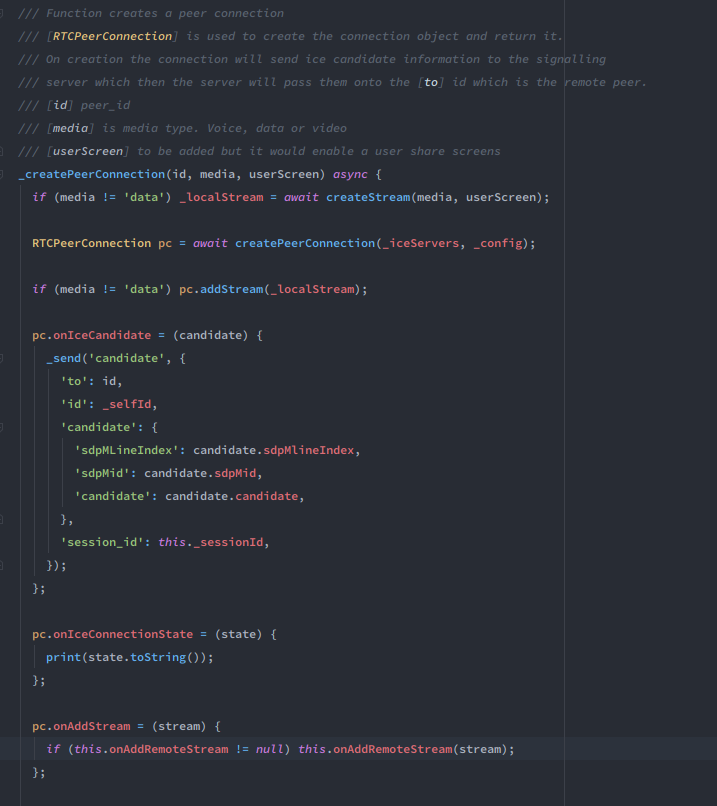
\includegraphics[width=1.0\textwidth]{images/connect_peer_function.png}
\end{figure}
Note the following in figure~\ref{image:peerConnectFunction}:
\begin{enumerate}
    \item A local stream is created using the media constraints defined in the createStream()
    \item A RTCPeerConnection is created passing it \_iceServers which is a map with a url of an iceserver and \_config which holds an optional argument to allow Chrome and Firefox to communicate.
    \item The \_localStream is added to the RTCPeerConnection as it holds information about the media of the local stream.
    \item The RTCPeerConnection is returned.
\end{enumerate}

When the peer connection is returned an offer is then made sending the SDP and media to the remote peer via the signalling server. See figure~\ref{image:createOfferFunc}
\begin{figure}[h!]
    \caption{Offer Creation}
    \label{image:createOfferFunc}
    \centering
    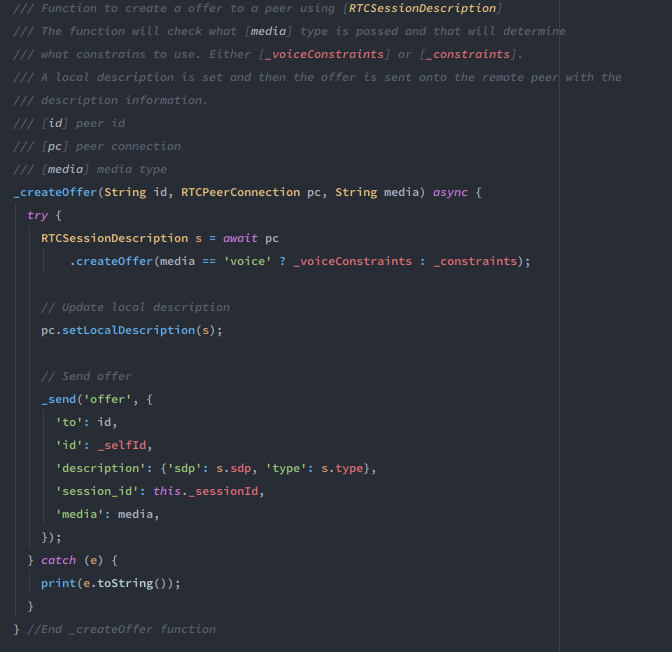
\includegraphics[width=1.0\textwidth]{images/create_offer_funtion.png}
\end{figure}

Once the remote peer receives the offer as in the figure below, a peer connection is created,
The remote description is set and finally the create answer function is called where that will send on its RTCSessionDescription to the peer that wishes to connect. One received both peers will be connected over their own encrypted connection. See figure~\ref{image:offerCaseCode}
\begin{figure}[h!]
    \caption{Offer Case Code Example}
    \label{image:offerCaseCode}
    \centering
    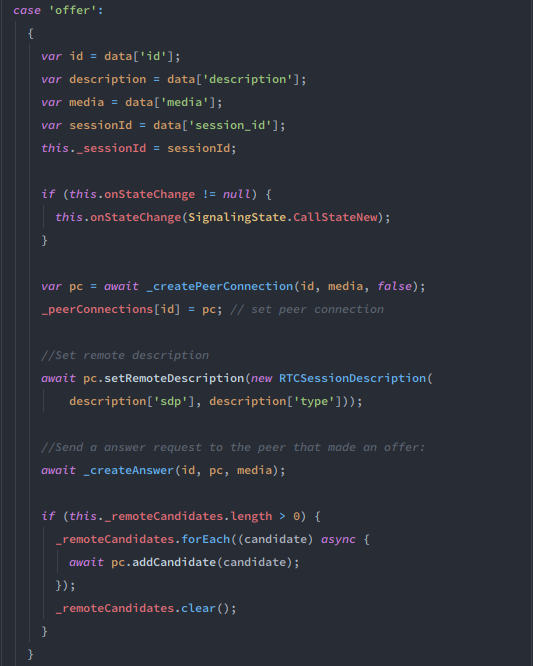
\includegraphics[width=1.0\textwidth]{images/offer_case_code.png}
\end{figure}

As previously discussed in  section~\ref{handleStateWebRTC}, all state is managed in the view class where a switch statement listens to signalling state in the callback function in the signaling class.
\\ Finally for WebRTC when a peer wishes to end a class with a remote peer a bye message is sent to the signaling server where that will send the message onto the remote peer as well as return it to the local peer so both peers can update their applications state and close the connection.  


\section{Database}
For vertex a MySQL was chosen as the application database. This was ultimately a big decision as the application could have used any assortment of SQL style databases, a noSQL database, or could have gone with a graph database, or possibly even a document store.
\\ This database uses an INNODB engine, which allows for full transaction support, various levels of locking, such as row-locking, and has full ACID compliance. The alternative which could have been used is a MYISAM engine, which supports different functionality which would not have suited the application.

\subsection{Schemas}
Due to the nature of the application only a handful of schemas were needed to handle the information saved throughout the application. The information being held is relatively straightforward. For each of the tables they need a unique identifier. In the case of schemas: User; Channel; Message; and Session; this was handled with the use of an auto-incrementing integer value, which increments by 1 per entry and starts at various values in respect to each table i.e. User will auto-increment from 100, Channel will auto-increment from 200 and so on. These auto-incrementing values are used in the form of the primary key for those tables with an alias of ‘id’ for each table allow for an ease of lookup, along with an O(1) time-complexity for look-up.
\\ The other remaining table, Member, uses foreign key values in a unique combination to handle look up, instead of a primary key value. For the most part, since there are few components of entry in each schema, the varaibles are given a ‘NOT NULL’ modifier, which means that data has to be given to them in order to avoid errors being raised.
\\ The database uses UTF-8 default as it’s character set, and utf8\_general\_ci as it’s collate set.
\\ The following schemas use cascading update, and cascading delete: Channel; Message; Session; Member. This allows for safe removal or modification of data, without setting null values.

\subsubsection{User Schema}
This schema handles the user information and was the first schema which had to be thought about.
\\ The User table is broken down into 3 components: ‘id’, ‘name’, ‘password’.
\\The ‘id’ of this table is described above, as an unsigned auto-incrementing integer starting at 100.
\\The ‘name’ is stored as a varchar of size 32 with a not-null modifier. This allows for an adequate size of allocated storage for the user name. The purpose of limiting the character is for memory preservation. The ‘name’ acts as a unique key to this schema. This is to avoid any duplication errors for any new users being inputted into the table, and also serves as a reference point should the ‘name’ need to be queried without explicitly knowing the ‘id’ beforehand. 
\\The ‘password’ is stored after it is hashed and salted using the bcrypt hashing function, which utilises the blowfish cipher. It is stored as a varchar of size 255 with a not null modifier.
See Figure~\ref{image:userSchema}

\subsubsection{Channel Schema}
This schema handles the channels being used in the application, and is broken down into 4 components.
\\The ‘id’ of this table is described above, as an unsigned auto-incrementing integer starting at 200.
The channel has to store a ‘name’ which forms part of a unique key used for referencing and duplication avoidance. This value is stored as a varchar of size 32 with a not null modifier.
\\It has a 'creator\_id', which acts as a foreign key from the User table (id).
\\It has a enumerated value, ‘type’, which allows us to differentiate between voice and text channels. This allows the user to create channels with a bit of variance to them.
\\Its unique key consists of ‘name’, ‘creator\_id’, and ‘type’ which serves as a way to avoid duplication's in the database.
See Figure~\ref{image:channelSchema}

\subsubsection{Message Schema}
This schema handles the messages being sent in the application. It is broken down into 5 components.
\\The first being the ‘id’. This is an unsigned auto-incrementing integer starting at 300.
\\The second being ‘channel’, which is a foreign key relating to the Channel table (see Channel for details). This serves as a way to link the message to the channel, without the messages spilling out into incorrect channels.
\\The third component is the ‘author’, which is a foreign key relating to the User table (see User for details). It serves as a way to link the message to the relevant user, without incorrect users seeing the data.
The fourth component is ‘content’. This is a varchar of size 255 with a not null modifier. This variable stores the message content that the user is sending.
\\The final component of this schema is the ‘timestamp’ for the message. This is stored as an Int of size 8 with a not null modifier.  The timestamp is stored as Unix Epoch time and the purpose of the size being set to 8 for this is to allocate enough space to handle epoch time correctly.
See Figure~\ref{image:messageSchema}

\subsubsection{Session Schema}
This schema handles the current session that is active for the user. It is a fairly straight-forward schema which consists of 3 components.
\\ The first component is the ‘id’. This is a varchar of size 255 with a not null modifier. The reason being is that the id should be stored as a UUID, therefore requiring an adequate amount of space allocation for the variable. This is the primary key for this table.
\\ The second component is ‘user’. This is a foreign key which links this table to the User table (see User for details).
The final component is ‘expire\_after’. This is another instance of Unix Epoch time, with a similar allocation of memory for this variable as was seen in the Message table. 
See Figure~\ref{image:sessionSchema}

\subsubsection{Member Schema}
The final table in this database is the Member table. This is responsible for grouping users with relevant channels, which allows for easier look-ups. It consists of 2 components, both of which are foreign keys.
\\ The first component is ‘channel’. This is set as an Integer of size 4, and is a  foreign key which relates to the Channel table on ‘id’.
\\ The second, and final component, is the ‘user’. This is also set as an Integer of size 4, and is a foreign key which relates to the User table on ‘id’.
\\ This table contains a unique key, which is comprised of  ‘channel’ and ‘user’. The reason being is to avoid duplicate entries in this schema, and also helps with look ups on the table.
See Figure~\ref{image:memberSchema}

\subsection{Testing}
In terms of testing, a full CRUD test is included in ‘vertex\_db\_v2.sql’, which is located on the database portion of the project repository. These tests verify correct functionality of creation of values, reading values, updating values, and deletion of values. They also verify and test for referential integrity for the database, along with duplication avoidance.

\begin{figure}[h!]
    \caption{User Schema}
    \label{image:userSchema}
    \centering
    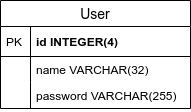
\includegraphics[width=0.3\textwidth]{images/UserSchema.png}
\end{figure}

\begin{figure}[h!]
    \caption{Channel Schema}
    \label{image:channelSchema}
    \centering
    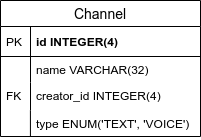
\includegraphics[width=0.3\textwidth]{images/ChannelSchema.png}
\end{figure}

\begin{figure}[h!]
    \caption{Message Schema}
    \label{image:messageSchema}
    \centering
    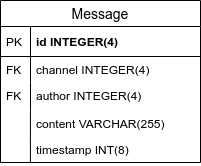
\includegraphics[width=0.3\textwidth]{images/MessageSchema.png}
\end{figure}

\begin{figure}[h!]
    \caption{Session Schema}
    \label{image:sessionSchema}
    \centering
    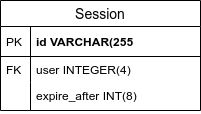
\includegraphics[width=0.3\textwidth]{images/SessionSchema.png}
\end{figure}

\begin{figure}[h!]
    \caption{Member Schema}
    \label{image:memberSchema}
    \centering
    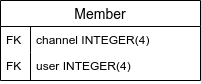
\includegraphics[width=0.3\textwidth]{images/MemberSchema.png}
\end{figure}

\begin{figure}[h!]
    \caption{Database Schema}
    \label{image:databaseSchema}
    \centering
    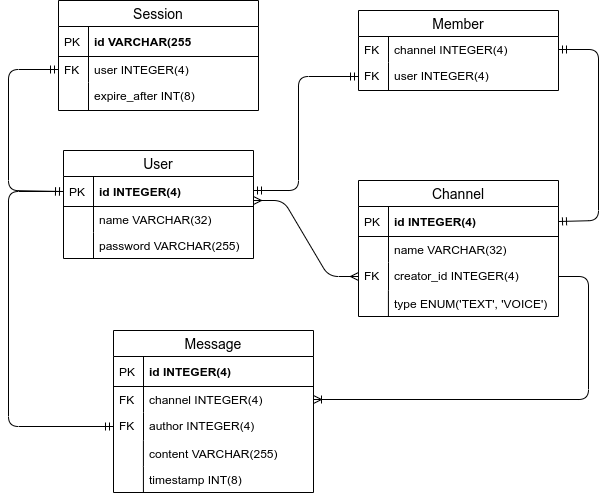
\includegraphics[width=1\textwidth]{images/FullSchemaDesign.png}
\end{figure}